\documentclass[10pt]{article}
\usepackage[letterpaper,top=0.34in,bottom=0.32in,left=0.55in,right=0.55in]{geometry}
\usepackage{graphicx}
\usepackage[hidelinks]{hyperref}
\usepackage{caption}
\usepackage{fontspec}
\setmainfont{texgyreheros-regular.otf}[BoldFont=texgyreheros-bold.otf,ItalicFont=texgyreheros-italic.otf,BoldItalicFont=texgyreheros-bolditalic.otf,Ligatures=NoCommon]
\setmonofont{Menlo}[Scale=0.85]
\urlstyle{same}
\hyphenation{checkpoint checkpoints}
\captionsetup{font={scriptsize},labelfont=bf,labelsep=period,skip=1pt}
\setlength{\parindent}{0pt}
\setlength{\parskip}{2pt}
\pagestyle{empty}
\begin{document}
\fontsize{7.8pt}{9.1pt}\selectfont

\noindent{\normalsize\bfseries Hearth on Pie - measurements on an iPhone 16 Pro}\hfill{\scriptsize Aarush Kandukoori, Carnegie Mellon University \quad November 8, 2026}

\textbf{Summary.} With Hearth's inferlet leaving a checkpoint after every reply, Pie started the next reply in
0.13 to 0.39\,s (median 0.22\,s) for chats of
633 to 3,794 tokens, while reading a 3,700 to
3,800-token chat from scratch took 7.7\,s on a cool phone and 10.5 to 11.2\,s on a warm one. The checkpoint rarely
survived reading another chat in between.

\textbf{Setup.} Every reply comes from Hearth's own Pie inferlet (Rust compiled to \texttt{wasm32-wasip3}) on Pie 0.6
(main \texttt{6168f02}), in-process on the Metal engine of an iPhone 16 Pro (A18 Pro, iOS 26.1) running Qwen3.5 2B
(4-bit, Gated DeltaNet plus attention). Two small iOS patches fix wasmtime's 2\,GiB growth reservation
and a state-slot commit that rounded past its reservation. Hearth gives Pie a 512\,MiB budget for its
KV pool and state slots together (1,496 KV pages of 16 tokens and 8 state
slots), 2 lanes, forward passes of at most 512 tokens and a 4,096-token context. The
inferlet reads a chat in two passes and asks Pie for a checkpoint of the recurrent state at the last
16-token page boundary before the prompt's final token. Pie keeps it in a state slot, so the next request
computes only what follows it. TTFT is timed inside the inferlet, from its start to the first sampled token (the app's
clock adds a median of 1.5\,ms). A
\emph{full re-read} is the same prompt with a unique tag at the start. Figures 1, 3 and 4a have
three trials per point, shuffled with a fixed seed. The main run's 134 requests ran back to back in
8 minutes with Low Power Mode off, and each records the thermal state iOS reported as it finished
(17 nominal, 83 fair, 34 serious).

\par\vspace{2pt}\noindent\begin{minipage}{\linewidth}\centering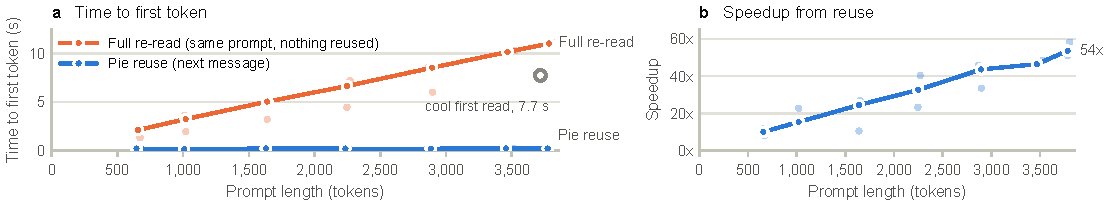
\includegraphics[width=\linewidth]{fig1_ttft_vs_length.pdf}
\captionof{figure}{TTFT against prompt length (a) and the speedup from reuse (b). A full re-read took
a median of 2.1\,s at about 660 tokens and 11.0\,s at
about 3,780, all three at ``fair''; the only read of 3,700 or more tokens at ``nominal'', a first read (hollow gray marker), took 7.7\,s. With reuse the inferlet computed
only the last 45 to 69 tokens and TTFT stayed at
0.13 to 0.31\,s (median 0.20\,s): 54x faster
than the re-read at about 3,780 tokens and 38x faster than the cool first read. Dots are trials; lines join medians.}
\end{minipage}
\par\vspace{2pt}\noindent\begin{minipage}{\linewidth}\centering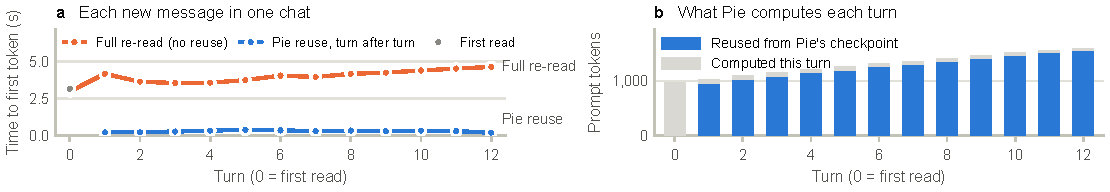
\includegraphics[width=\linewidth]{fig2_multiturn.pdf}
\captionof{figure}{One chat carried on for 12 more turns (turn 0, gray, is its first read;
the prompt grows from 966 to 1,602 tokens). (a) Every reuse turn
started in 0.19 to 0.39\,s while a
full re-read grew from 3.0 to 4.6\,s. (b) Each turn computed
only its last 34 to 80 tokens
(12 of 12 reused the previous checkpoint), 1,723 of the chat's
17,051 prompt tokens in all.}
\end{minipage}
\par\vspace{2pt}\noindent\begin{minipage}{\linewidth}\centering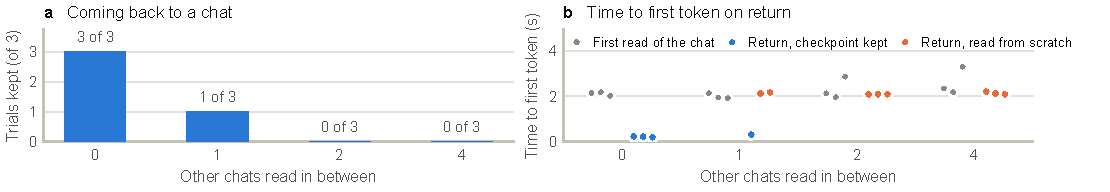
\includegraphics[width=\linewidth]{fig3_retention.pdf}
\captionof{figure}{Coming back to a chat after reading \emph{K} other new chats (three trials per \emph{K}).
(a) The checkpoint was still there in 3 of 3 trials with \emph{K} = 0, 1 of 3 with \emph{K} = 1 and none with \emph{K} = 2 or 4. A surviving checkpoint covered 92\% of the returning
prompt. (b) Returns without it took a median of 2.1\,s, about the same as the first
reads of those eight chats (2.2\,s). A Low Power Mode run (one trial per \emph{K}) kept it at \emph{K} = 0 and lost it at \emph{K} = 1, 2, 3, 4 and 6.}
\end{minipage}
\par\vspace{2pt}\noindent\begin{minipage}{\linewidth}\centering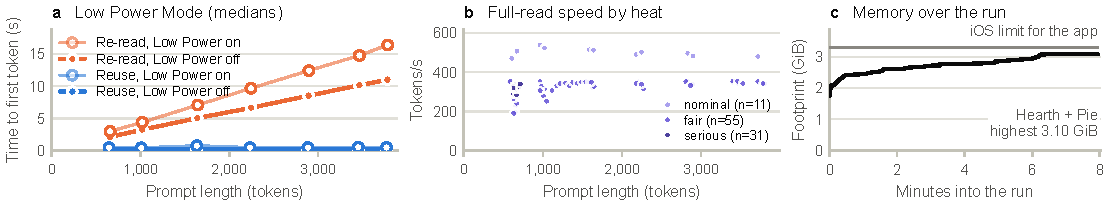
\includegraphics[width=\linewidth]{fig4_power_heat_memory.pdf}
\captionof{figure}{(a) A separate, earlier run with Low Power Mode on, the phone at
``nominal'': full re-reads ran at about 232 tokens/s against about 492 at ``nominal'' with it off,
and reuse medians stayed at 0.42 to 0.75\,s. The
Low Power off lines are the main run, mostly at ``fair''. (b) Full-read speed by length and thermal state. Reads of
2,000 or more tokens ran at a median of 492 tokens/s at ``nominal''
(n~=~5) and 344 at ``fair'' (n~=~19). Most short ``fair'' reads (10 of 14) come from the slow stretch of requests 90 to 100, so ``fair'' and ``serious'' are not compared.
Reuse barely changed with heat (medians 0.19 to 0.22\,s). (c) The app's memory
footprint (\texttt{phys\_footprint}) rose from 1.75\,GiB before the first request to
3.10\,GiB, flat from minute 6.3 on, 0.20\,GiB
under the iOS limit for the app (3.30\,GiB).}
\end{minipage}

\par\vspace{2pt}\textbf{What this suggests.}
\textbf{Keeping checkpoints across chats is the main gap I found.} In this configuration (8 state slots,
512\,MiB), reading one other chat usually discarded a chat's checkpoint and reading two or more always
did; this run did not log which path dropped them, which I want to trace next. Pie's Metal engine already has a disk
tier for parked KV and state, so keeping checkpoints there could carry reuse across chats.
\textbf{Memory headroom on iOS is small.} With
the 512\,MiB budget the footprint still grew 1.35\,GiB, more than the
budget itself, and came within 0.20\,GiB of the limit; I have not broken that growth down yet. An earlier build that left pool sizes to Pie's working-set hint (5,042 KV pages, 4 lanes) and lacked the state-slot fix ended with signal 9 after 14 replies, shortly after that commit failed once (144\,MiB asked of a 142.5\,MiB reservation).
\textbf{Pie's Neural Engine path did not run.} Its programs failed to compile here
(\mbox{``Operation not permitted''}), so the GPU ran every layer; decode ran at a median of
38 tokens/s (97 replies of 16
to 24 tokens).

\textbf{Limitations.} One phone and one model; the Low Power Mode run and the earlier build are separate runs. Each
re-read ran right after its reuse request, on a slightly warmer phone, and the first trial's shuffle came out nearly in
ascending order. The phone reported unplugged for requests 87 to 90, and seven of the eight slowest full reads came from requests 90 to 100. Pie ran its
checked-in GPU profile (\texttt{apple9.toml}), never measured on the A18 Pro. Data, analysis and the sweep are at \href{https://github.com/aarushkandukoori/hearth/tree/main/research/2026-11-08-iphone}{\nolinkurl{github.com/aarushkandukoori/hearth/tree/main/research/2026-11-08-iphone}}.

\end{document}
